\documentclass{article}
\usepackage{amsmath}
\usepackage{geometry}
%\usepackage[]{mcode}
\usepackage{graphicx}
\usepackage{float}
\usepackage{placeins}
\usepackage{gensymb}

\geometry{
left = 1.25in,
lmargin = 1.25in,
inner = 1.25in,
right = 1.25in,
rmargin = 1.25in,
outer = 1.25in,
top = 1in,
tmargin = 1in,
bottom = 1in,
bmargin = 1in,
}

\begin{document}

\title{Inverted Pendulum Controllers}
\author{Garrett Wilson and Nathan Zimmerly \\ \\
ENGR 352}
\maketitle

\clearpage

\tableofcontents

\pagebreak

\section{PID Controller}
\subsection{Transfer Function of $\theta$ / F Without Friction Derivation}
Below is the derivation of the transfer function with an input of F and an output of $\theta$.


\begin{equation} 
\label{eqn1}
\ddot \theta (I+m y_c^2)+\ddot x (m y_c)+b \dot \theta - m g y_c \theta = 0 
\end{equation}


\begin{equation} 
\label{eqn2}
\ddot \theta(m y_c) + \ddot x(M+m) = F
\end{equation}

%\\
Laplace transforms of equations \ref{eqn1} and \ref{eqn2} gives

\begin{equation} 
\label{eqn1l}
\theta (I+m y_c^2) s^2+ X (m y_c) s^2+b \theta s - m g y_c \theta = 0 
\end{equation}


\begin{equation}  
\label{eqn2l}
\theta (m y_c) s^2+ X (M+m) s^2= F
\end{equation}

%\\
Next, solving \ref{eqn2l} for x and substituting it into \ref{eqn1l}

\begin{equation}  
\label{eqn2lb}
X = \frac{F - \theta (m y_c) s^2}{(M+m) s^2}
\end{equation}

\begin{equation} 
\label{eqn3}
\theta (I+m y_c^2) s^2+ \frac{(F - \theta (m y_c) s^2)(m y_c) s^2}{(M+m) s^2} + b \theta s - m g y_c \theta = 0 
\end{equation}

Simplifying \ref{eqn3} leads to


\begin{equation} 
\label{eqn3}
\theta (I+m y_c^2) s^2+ \frac{F m y_c}{(M+m)} -\frac{\theta (m y_c)^2 s^2}{(M+m)} + b \theta s - m g y_c \theta = 0 
\end{equation}

\begin{equation} 
\label{eqn3b}
\theta [(I+m y_c^2) s^2 - \frac{(m y_c)^2 s^2}{(M+m)} + b s - m g y_c] +\frac{F m y_c}{(M+m)}  = 0 
\end{equation}

\begin{equation} 
\label{eqn3c}
\theta [(I+m y_c^2) s^2 - \frac{(m y_c)^2 s^2}{(M+m)} + b s - m g y_c] = -\frac{F m y_c}{(M+m)} 
\end{equation}

\begin{equation} 
\label{eqn3d}
\theta [(I+m y_c^2)(M+m) s^2 - (m y_c)^2 s^2 + b s (M+m) - m g y_c (M+m) ] = -F m y_c
\end{equation}

\begin{equation} 
\label{eqn3e}
\frac{\theta}{F} = \frac{-m y_c}{(I+m y_c^2)(M+m) s^2 - (m y_c)^2 s^2 + b s (M+m) - m g y_c (M+m)}
\end{equation}

\begin{equation} 
\label{eqntf1}
\frac{\theta}{F} = \frac{-m y_c}{[(I+m y_c^2)(M+m) - (m y_c)^2]s^2 + b (M+m) s - m g y_c (M+m)}
\end{equation}

Equation \ref{eqntf1} is the transfer function of $\theta$ / F without friction.

\subsection{Transfer Function X / $\theta$ Derivation}

Using \ref{eqn1l}

\begin{equation} 
\label{eqn4}
X (m y_c) s^2 = -\theta [(I+m y_c^2) s^2+b s - m g y_c] = 0 
\end{equation}

\begin{equation} 
\label{eqntf2}
\frac{X}{\theta} = \frac{-[(I+m y_c^2) s^2+b s - m g y_c]}{(m y_c) s^2} 
\end{equation}

Equation \ref{eqntf2} is the transfer function of X / $\theta$.



\subsection{Transfer Function of $\theta$ / F with Friction Derivation}

Below is the derivation of the transfer function with an input of F and an output of $\theta$.

\begin{equation} 
\label{eqn5}
\ddot \theta (I+m y_c^2)+\ddot x (m y_c)+b \dot \theta - m g y_c \theta = 0 
\end{equation}

\begin{equation} 
\label{eqn6}
\ddot \theta(m y_c) + \ddot x(M+m) = F+ F_{fric}
\end{equation}

These equations are equivalent to \ref{eqn1} and \ref{eqn2} except \ref{eqn2} has $F_{fric}$ added.

\begin{equation}
\label{eqn7}
F_{fric} = - b_cart \dot x
\end{equation}

Substituting \ref{eqn7} into \ref{eqn6}

\begin{equation} 
\label{eqn8}
\ddot \theta(m y_c) + \ddot x(M+m) = F - b_{cart} \dot x
\end{equation}

Laplace Transforms of \ref{eqn5} and \ref{eqn8} give

\begin{equation} 
\label{eqn5l}
\theta (I+m y_c^2) s^2+ X (m y_c) s^2+b \theta s - m g y_c \theta = 0 
\end{equation}

\begin{equation} 
\label{eqn8l}
\theta (m y_c) s^2+ X (M+m) s^2= F - b_{cart} X s
\end{equation}

Solving \ref{eqn8l} for X and solving substituting the result into \ref{eqn5l} gives

\begin{equation} 
\label{eqn8lb}
X [(M+m) s^2 + b_{cart} s]= F - \theta(m y_c) s^2
\end{equation}

\begin{equation} 
\label{eqn8lc}
X = \frac{F - \theta(m y_c) s^2}{(M+m) s^2 + b_{cart} s}
\end{equation}

\begin{equation} 
\label{eqn9}
\theta (I+m y_c^2) s^2+  \frac{[F - \theta(m y_c) s^2] m y_c s^2}{(M+m) s^2 + b_{cart} s}+b \theta s - m g y_c \theta = 0 
\end{equation}

Solving \ref{eqn9} for the transfer function

\begin{multline} 
\label{eqn9b}
\theta (I+m y_c^2) s^2 [(M+m) s^2 + b_{cart} s]+ F m y_c s^2 - \theta(m y_c)^2 s^4 \\ 
+ b \theta s [(M+m) s^2 + b_{cart} s]- m g y_c \theta [(M+m) s^2 + b_{cart} s]= 0 
\end{multline}

\begin{multline} 
\label{eqn9c}
\theta [(I+m y_c^2) s^2 ((M+m) s^2 + b_{cart} s) - (m y_c)^2 s^4 + b s ((M+m) s^2 \\+ b_{cart} s)
- m g y_c ((M+m) s^2 + b_{cart} s)] = -F m y_c s^2
\end{multline}

\begin{multline} 
\label{eqn9d}
\frac{\theta}{F} = (-m y_c s^2)/((I+m y_c^2) s^2 ((M+m) s^2 + b_{cart} s) - (m y_c)^2 s^4 + b s ((M+m) s^2 + b_{cart} s) \\
- m g y_c ((M+m) s^2 + b_{cart} s))
\end{multline}

\begin{multline} 
\label{eqn9e}
\frac{\theta}{F} = (-m y_c s^2)/((I+m y_c^2) s^2 ((M+m) s^2 + b_{cart} s) - (m y_c)^2 s^4 + b s ((M+m) s^2 + b_{cart} s) \\
- m g y_c ((M+m) s^2 + b_{cart} s))
\end{multline}

\begin{multline} 
\label{eqn9f}
\frac{\theta}{F} = (-m y_c s)/(s^3(m M y_c^2 + I m + I M) + s^2(b m + b M + I b_{cart} + m b_{cart} y_c^2) + s(b b_{cart} \\
- g m^2  y_c - g m M y_c) - g m b_{cart} y_c)
\end{multline}

Equation \ref{eqn9f} is the transfer function of $\theta$ / F with friction.

%\clearpage


\subsection{Figures}
%\\ 
%\\

\begin{figure}[!htb]
    \centering
    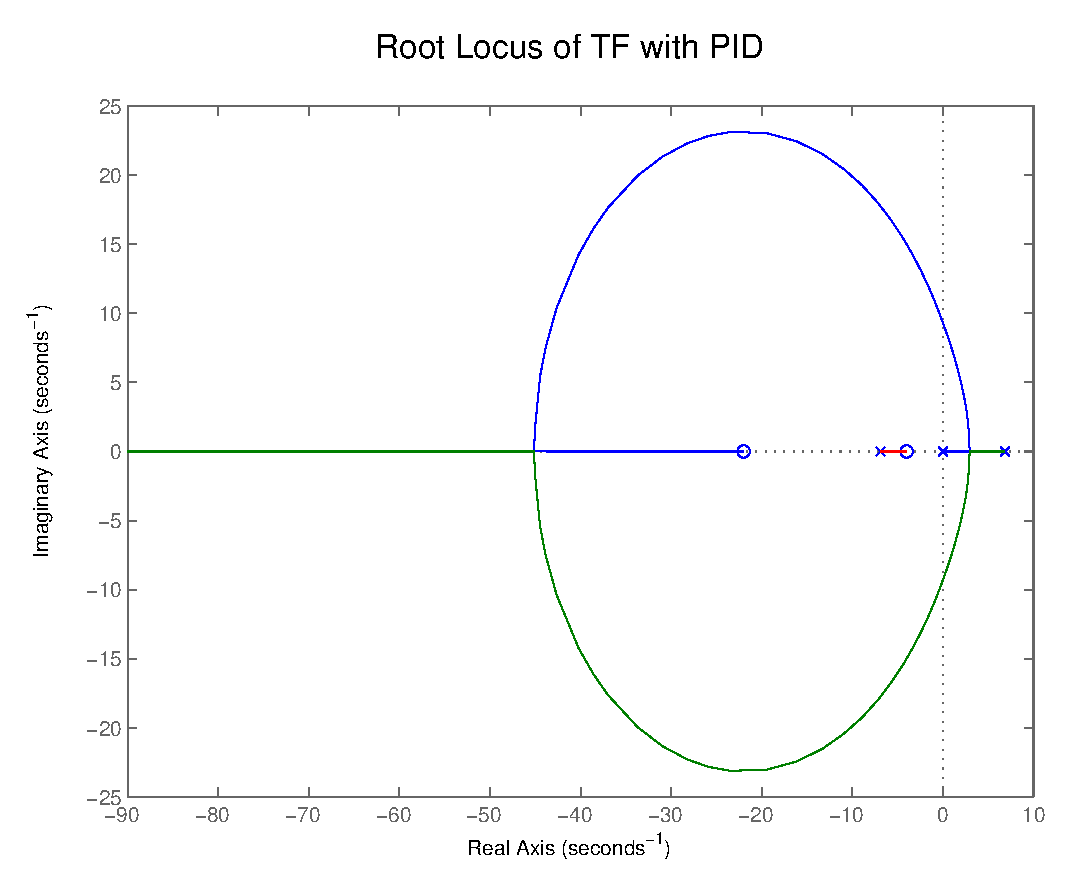
\includegraphics[scale=0.6]{1}
    \caption{ Rlocus of TF with PID Controller}
\end{figure} 

\begin{figure}[!htb]
    \centering
    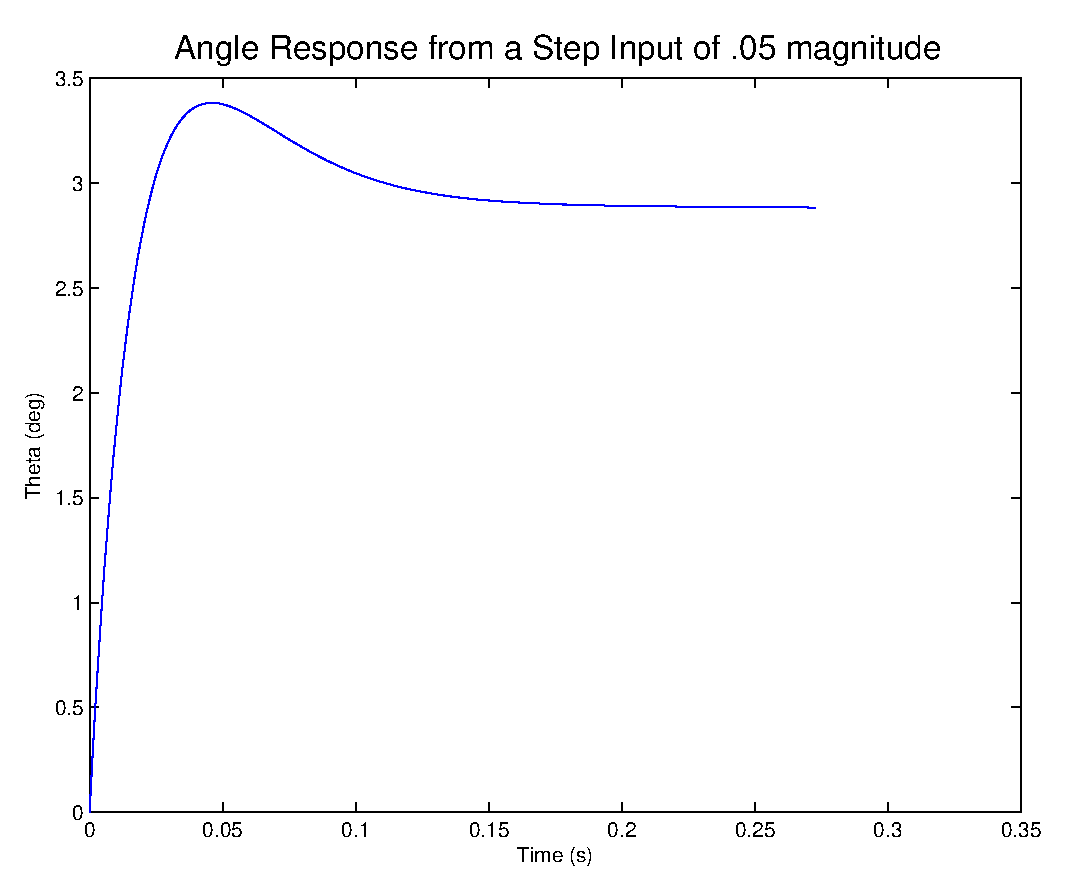
\includegraphics[scale=0.6]{2}
    \caption{Angle Response for a Step Input ($\theta_0$ = 0$^{\circ}$)}
\end{figure} 

\begin{figure}[!htb]
    \centering
    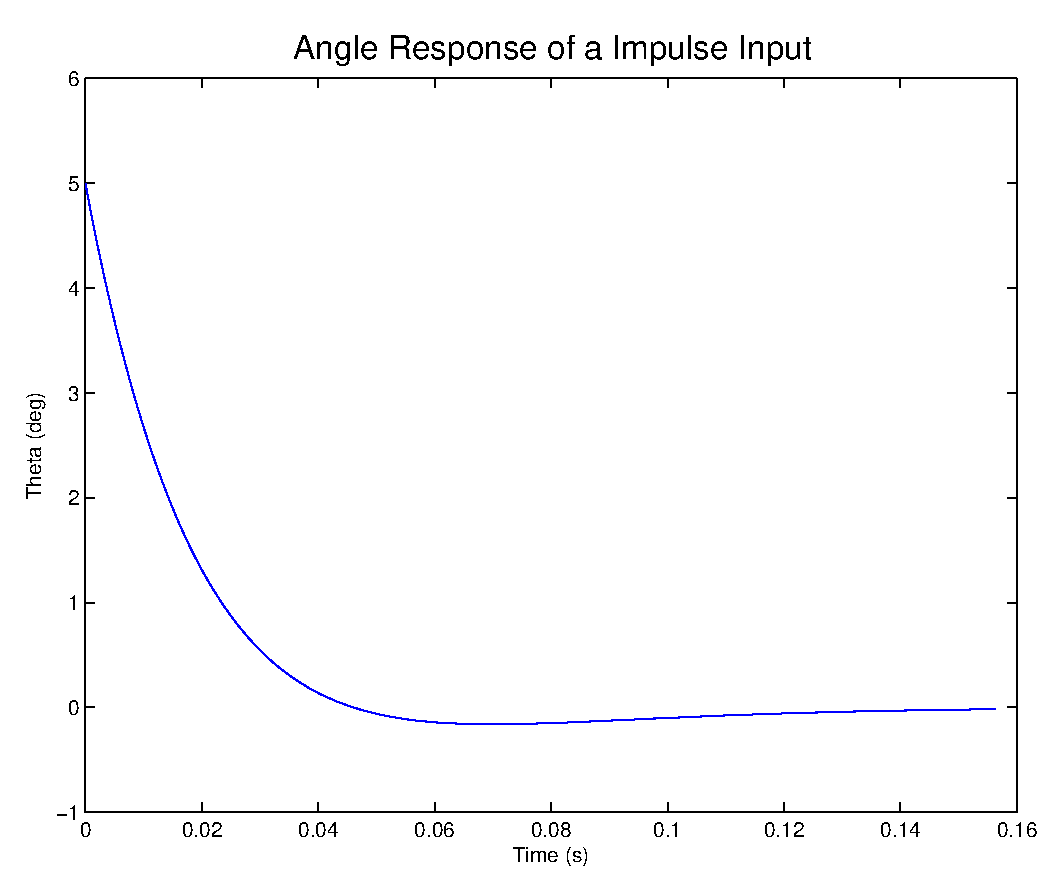
\includegraphics[scale=0.6]{3}
    \caption{Angle Response for an Impulse Input ($\theta_0$ = 5$^{\circ}$)}
\end{figure} 

\begin{figure}[!htb]
    \centering
    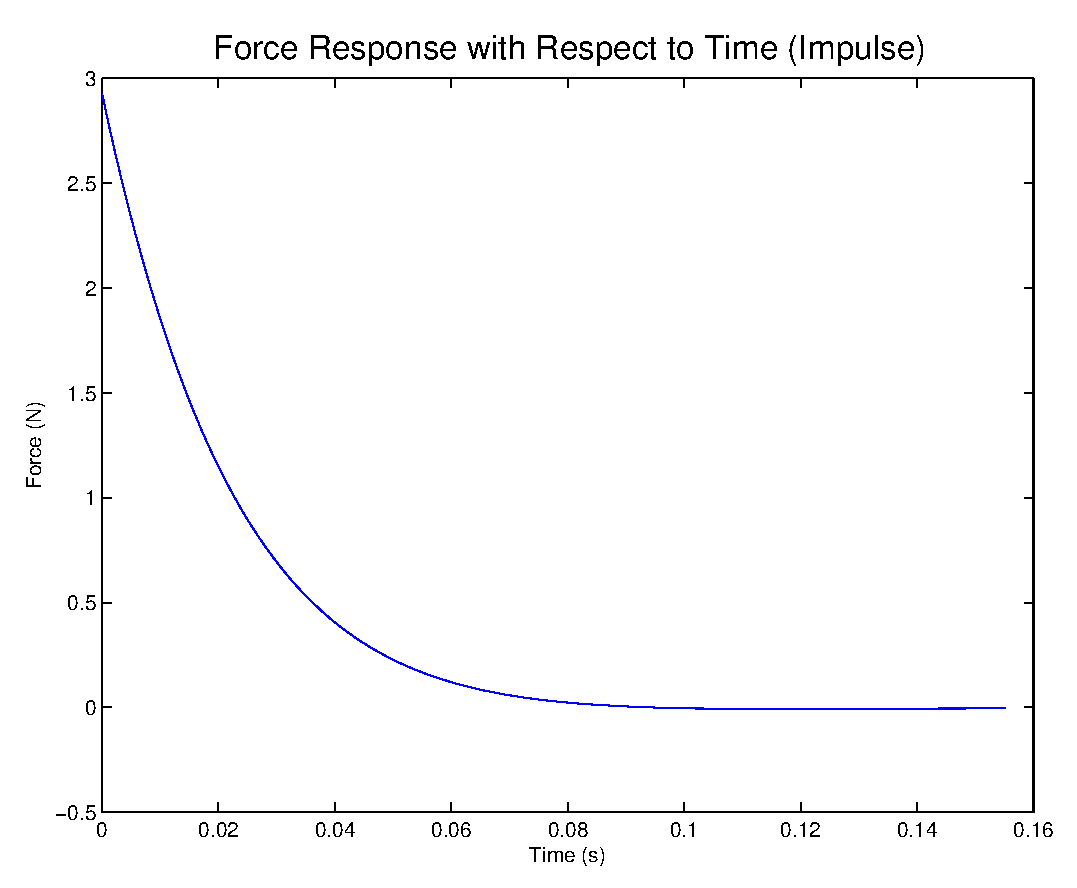
\includegraphics[scale=0.6]{4}
    \caption{Force Response of an Impulse Input ($\theta_0$ = 5$^{\circ}$)}
\end{figure} 

\begin{figure}[!htb]
    \centering
    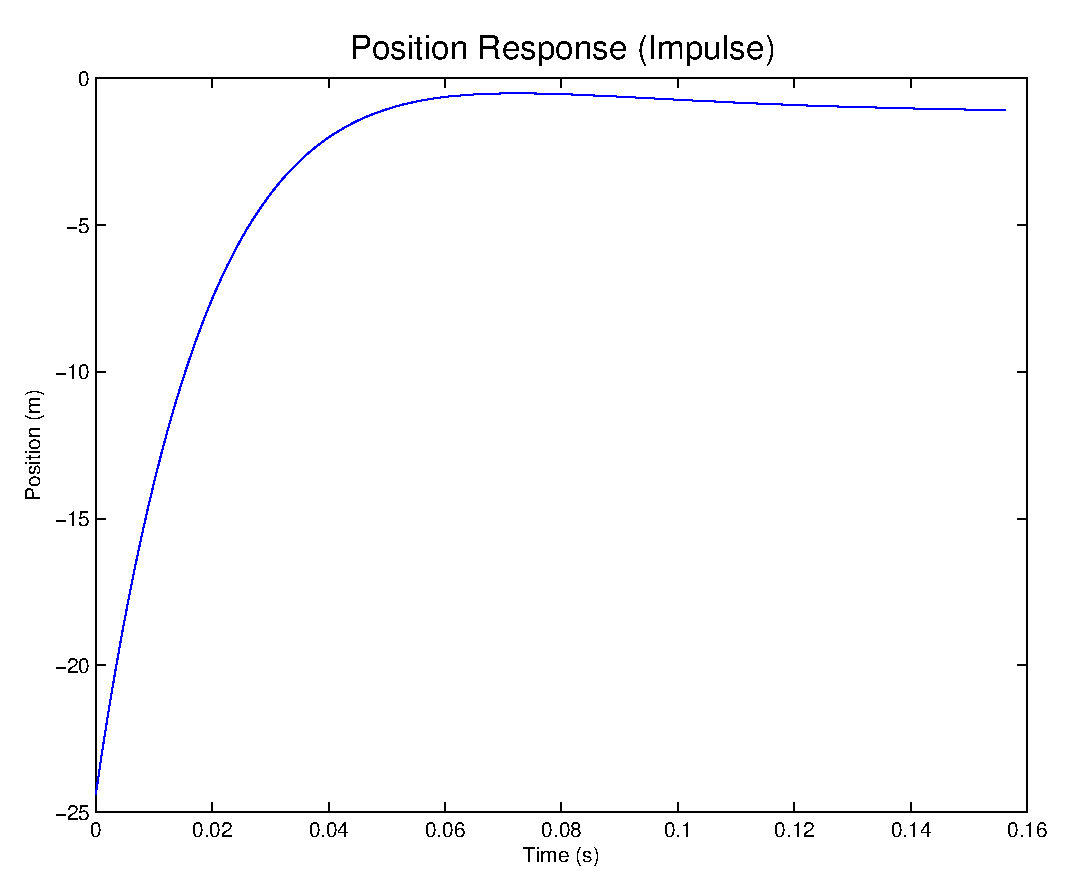
\includegraphics[scale=0.6]{5}
    \caption{Position Response of an Impulse Input ($\theta_0$ = 5$^{\circ}$)}
\end{figure} 

\begin{figure}[!htb]
    \centering
    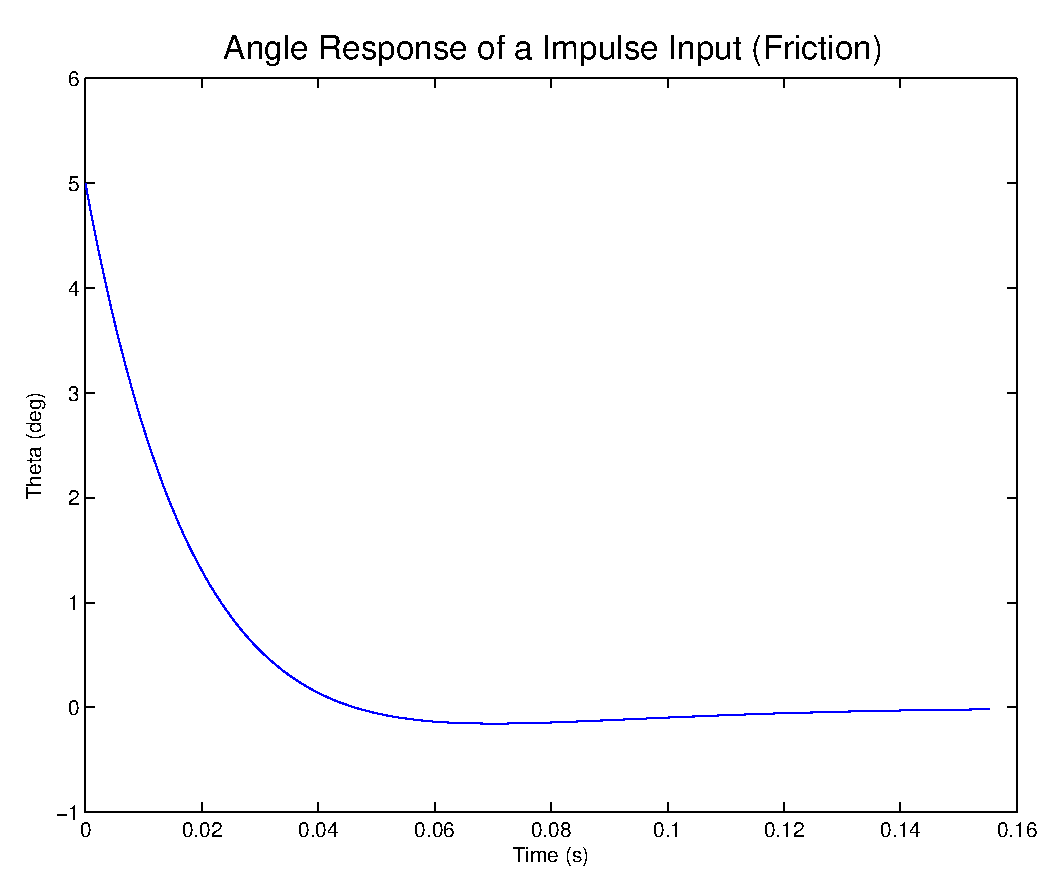
\includegraphics[scale=0.6]{6}
    \caption{Angle Response of an Impulse Input with Friction ($\theta_0$ = 5$^{\circ}$)}
\end{figure} 

\begin{figure}[!htb]
    \centering
    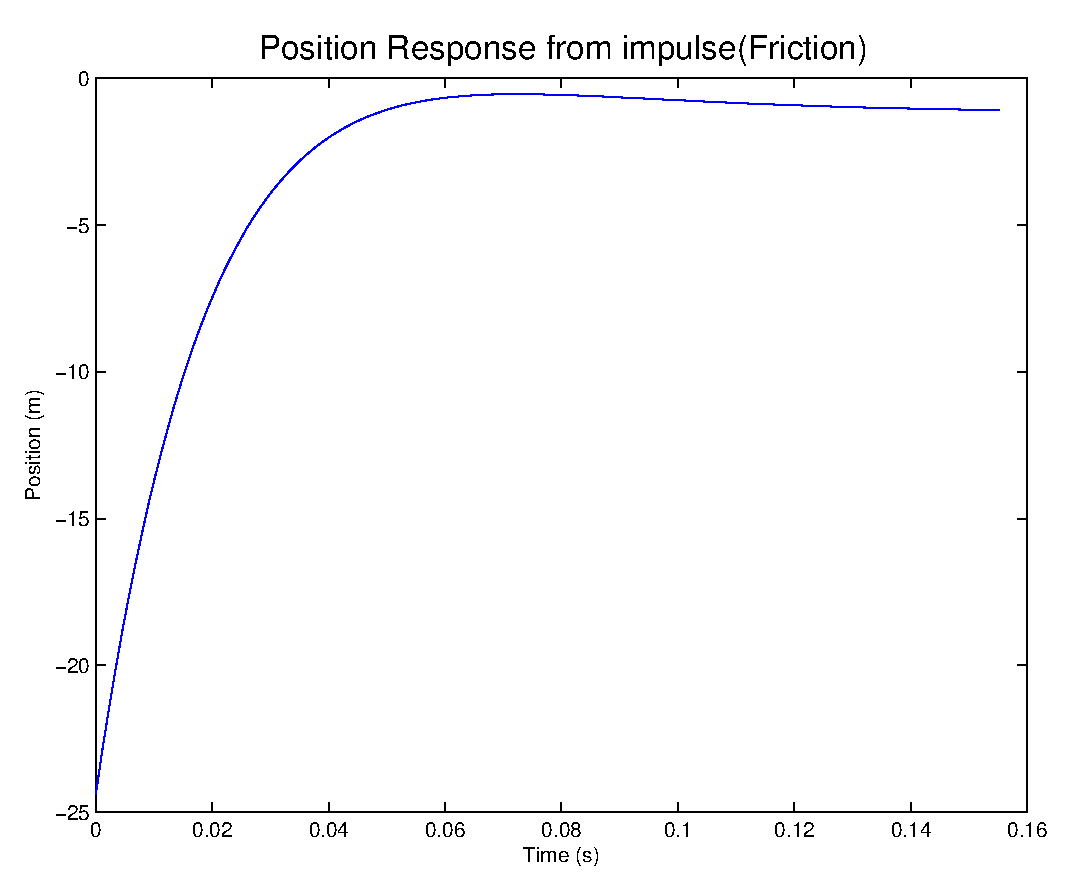
\includegraphics[scale=0.6]{7}
    \caption{Position Response of an Impulse Input with Friction ($\theta_0$ = 5$^{\circ}$)}
\end{figure} 

\FloatBarrier

\subsection{Discussion}

\subsubsection{Requirements}

My controller is stable, has 0\% steady state error for step inputs, a settling time that is .292s of the maximum, an overshoot that is 51.4\% of the maximum, and a force that is 97.7\% below the maximum. All of these values are quite satisfying except for the force that is used. I think that if I had more time, I could adjust the poles for a better value. Note that a step input is impractical for the angle because we want it to be straight up. An impulse force is much more practical for the real world.

\begin{center}
\begin{tabular}{|c | c | c|} 
\hline
 & Goal & Actual \\ 
\hline
Stability &  Stable & Stable \\ 
\hline
Steady State Error (step input)  & 0\% & 0\% \\ 
\hline
Settling Time (Max) & .5 s & .146 s \\
\hline
Overshoot (Max)& 35\% & 18.1\% \\
\hline
Force (Max) & 3N & 2.929N \\
\hline
\end{tabular}
\end{center}

\subsubsection{Friction}

Accounting for friction kept all my parameters the same or improved them except for the force used. This makes sense because it would take a larger force to overcome friction and move the pendulum the same distance. I am unsure of why the settling time and overshoot improved, my guess is that it is because the friction slows down the cart so that it the overshoot is less and the settling time improves because of this. The position response seems to be the same whether friction is accounted for or not. This is interesting because I thought that friction would slow down the cart until it stopped, but it keeps moving as long as the simulation runs. My current theory on this is that the model controls the position, so even if friction is added, the model is going to add more force to overcome the friction.

\begin{center}
\begin{tabular}{|c | c | c | c|} 
\hline
 & Goal & Actual & Actual (With Friction)\\ 
\hline
Stability &  Stable & Stable & Stable\\ 
\hline
Steady State Error (step input)  & 0\% & 0\% & 0\%\\ 
\hline
Settling Time (Max) & .5 s & .146 s & .143 s \\
\hline
Overshoot (Max)& 35\% & 18.1\% & 17.3\% \\
\hline
Force (Max) & 3N & 2.929N & 2.97N\\
\hline
\end{tabular}
\end{center}

\section{LQR State Space Controller}
\subsection{4th Order}
\subsubsection{State-Space Modeling}
Below is the free-body diagram of the inverted pendulum and cart

\begin{figure}[!htb]
\centering
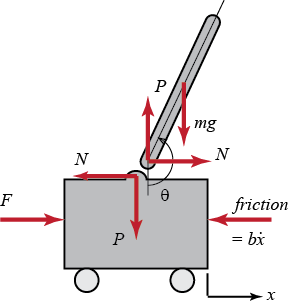
\includegraphics{pendulumfbd}
\caption{Source: http://ctms.engin.umich.edu/}
\end{figure}

Summation of carts forces in the horizontal direction
\begin{equation} 
\label{eqn1}
F = M\ddot{x}+b\dot{x} + N
\end{equation}

Summation of the pendulum forces in the horizontal direction
\begin{equation} 
\label{eqn2}
N = m\ddot{x}+m l \ddot{\phi} cos(\phi)-m l \dot{\phi}^2sin(\phi)
\end{equation}

Substituting \ref{eqn2} into \ref{eqn1}
\begin{equation} 
\label{eqn3}
F = M\ddot{x}+b\dot{x} + m\ddot{x}+m l \ddot{\phi} cos(\phi)-m l \dot{\phi}^2sin(\phi)
\end{equation}

Next, the sum of forces perpendicular to the pendulum
\begin{equation} 
\label{eqn4}
Psin(\phi)+Ncos(\phi)-mgsin(\phi) = m l \ddot{\phi} + m\ddot(x)cos(\phi)
\end{equation}

Summing tthe moments about the centroid of the pendulum
\begin{equation} 
\label{eqn5}
-P sin(\phi)-N cos(\phi) = I \ddot{\phi}/l
\end{equation}

Combining \ref{eqn4} and \ref{eqn5} leads to 
\begin{equation} 
\label{eqn6}
(I+m l^2)\ddot{\phi} + m g lsin(\phi) = -m l \ddot{x} cos(\phi)
\end{equation}

Small angle approximations. $\theta$ replaces $\phi$ so that the angle $\theta$ = 0 $\degree$ is straight up.
\\

\begin{equation} 
\label{sa1}
cos(\phi) = cos(\pi + \theta) \approx -1
\end{equation}

\begin{equation} 
\label{sa2}
sin(\phi) = sin(\pi + \theta) \approx -\theta
\end{equation}

\begin{equation} 
\label{sa3}
\dot{\phi} = \dot{\theta} \approx 0
\end{equation}

Plugging \ref{sa1} and \ref{sa2} into \ref{eqn3} and \ref{eqn6} leads to
\begin{equation} 
\label{eqn3b}
F = (M+m)\ddot{x}+b\dot{x} -m l \ddot{\theta}
\end{equation}

\begin{equation} 
\label{eqn6b}
(I+m l^2)\ddot{\theta} - m g l\theta = m l \ddot{x}
\end{equation}

Motor Equations
\begin{equation} 
\label{eqn7}
L i + R i = V - k_m\dot{\theta}
\end{equation}

\begin{equation} 
\label{eqn8}
\tau = k_m*i
\end{equation}
To arrive at state space equations add \ref{eqn7} and \ref{eqn8} into \ref{eqn3b} and \ref{eqn6b}. Note: L = 0.

Plugging \ref{eqn8} into \ref{eqn7} leads to 
\begin{equation} 
\label{eqn9}
F = \frac{R k_m}{r(V-k_m\dot{\theta})}
\end{equation}

Finally, plugging \ref{eqn9} into \ref{eqn3b} and \ref{eqn6b} and solving for $\ddot{x}$ and $\ddot{\theta}$ leads to the state space equations below

\begin{equation}
\label{ss1}
\begin{bmatrix}
\dot{x}\\
\ddot{x}\\
\dot{\theta}\\
\ddot{\theta}\\
\end{bmatrix} =
\begin{bmatrix}
0&1&0&0\\
0&\frac{(I+m l^2)/(m l) (-(b+K^2/(R r^2))}{(M+m) (I+m l^2)/(m l)-m l}&\frac{(I+m l^2)/(m l) (M+m) g}{[(M+m) 		(I+m l^2)/(m l)-m l]-g}&0\\
0&0&0&1\\
0&\frac{-(b+K^2/(R r^2))}{(M+m) (I+m l^2)/(m l)-m l}&\frac{(M+m) g}{(M+m) (I+m l^2)/(m l)-m l}&0\\
\end{bmatrix}
\begin{bmatrix}
x\\
\dot{x}\\
\theta\\
\dot{\theta}\\
\end{bmatrix} +
 	\begin{bmatrix}
0\\
\frac{(I+m*l^2)/(m*l)*(K/(R*r)}{(M+m) (I+m l^2)/(m l)-m l}\\
0\\
\frac{K/(R*r)}{(M+m) (I+m l^2)/(m l)-m l}\\
\end{bmatrix} v
\end{equation}
  
\begin{equation}
\label{ss2}
\begin{bmatrix}
x\\
\theta \\
\end{bmatrix} =
\begin{bmatrix}
1&0&0&0\\
0&0&1&0\\
\end{bmatrix}
\begin{bmatrix}
x\\
\dot{x}\\
\theta\\
\dot{\theta}\\
\end{bmatrix}
\end{equation}

\subsubsection{Poles, Stability, and Observability}
Now that the state-space equations are found, the poles of the model are equal to the eigen values of the A matrix. The original Poles are shown below:
\begin{enumerate}
  \item   0.00000 + 0.00000i
  \item -9.9916 + 0.00000i
  \item -4.9981 + 0.00000i
  \item 5.1345 + 0.00000i
\end{enumerate}
Because one of the poles is positive, the system is unstable. We will fix this with a controlled matrix A in the next section.

If the rank of the controllability matrix shown below equals the number of states the system (n) is made up of, then the system is controllable. In our case the rank of R equals 4 so our system is controllable. This means that our system can reach any state.

\begin{equation} 
\label{ctrb}
\centering
R = \begin{bmatrix}
	B&AB&\hdots&A^{n-1}B\\
	\end{bmatrix}
\end{equation}
 
 If the rank of the observability matrix shown below equals the number of states the system is made up of, then the system is observable. In our case the rank of O eqauls 4 so our system is observable. This means that in any possible situation, the current state of our system can be determined using only the outputs.
 
 \begin{equation} 
\label{obsv}
\centering
O = \begin{bmatrix}
	C\\
	CA\\
	\vdots\\
	CA^{n-1}\\
	\end{bmatrix}
\end{equation}

\subsubsection{LQR Controller}
A linear-quadratic regulator (LQR) weights factors depending on their importance using the nxn Q matrix, while minimizing another factor using the variable R. In our case, the weighted factors were the position of the cart (x) and the angle of the pendulum ($\theta$). Also, the factor that we minimized is the velocity of the cart. A good starting point for Q is C'C evenly weighting the factors. However, we care much more about the pendulum staying vertical than we do the position staying at 0 m. Because of this, after some tests we weighted x at 1000 and $\theta$ at 100,000. leaving the Q matrix below. Also, a good place to start the limiting factor is 1, but we change R = 0.1.

 \begin{equation} 
\label{q}
\centering
Q = \begin{bmatrix}
	1000&0&0&0\\
	0&0&0&0\\
	0&0&100,000&0\\
	0&0&0&0\\
	\end{bmatrix}
\end{equation}

In LQR controllers, the state-feedback control gains vector k is used to move the poles in the system. It can be calculated by minimizing the cost function J. We used Octave's LQR function to calculate our k vector. Once calculated, the corrected A matrix can be calculated using the equation below.

\begin{equation}
\label{ac}
A_c=[A-Bk]
\end{equation}

\subsubsection{Precompensator}
At this point, our pendulum seemed to stay up, but the cart would not stay at the center. Because of this, we had to add a precompensator to account for steady-state error. Because the cart's position had steady-state error, we chose the C matrix below.
\\

\begin{equation}
\label{pcomp}
\centering
C_n = [1 0 0 0]
\end{equation}
 
 By replacing the state space C matrix with C\_n, $\bar{N}$ can be calculated. We used Octave's rscale function to calulate $\bar{N}$. $\bar{N}$ is a scale factor that eliminates the stead-state error of a system to a step input. It should be noted that $\bar{N}$ only works for single input systems, which is why we could use it to only eliminate the steady state error in the carts position. Once $\bar{N}$ is calculated, the state space equation uses the corrected A matrix, B $\bar{N}$, C, and D for the A, B, C, and D matrices respectively.
 
 \subsubsection{Adding an Observer-Based Estimator}
 Previous work assumes full-state feedback, which means that x, $\dot{x}$, $\theta$, and $\dot{\theta}$ are all being measure. However, only x and $\theta$ are being measured so we must add observer based control. Below are the previous block diagram, and the updated block diagram with the observer-based estimator.

\begin{figure}[!htb]
\centering
  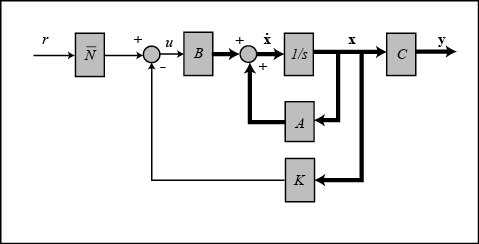
\includegraphics[width=.7\linewidth]{blockd}
  \caption{Original}
  \label{bd}
  \end{figure}

\begin{figure}[!htb]
\centering
  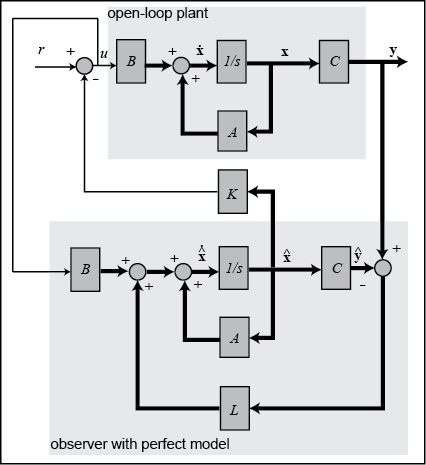
\includegraphics[width=.6\linewidth]{observer_blockd}
  \caption{With Precompensator}
  \label{bd2}
\end{figure}


\clearpage

The speed of convergence depends on the poles of the estimator. Since we are going to use the estimation before the actual event accurs, we want the estimation to converge must faster. Because of this we want the poles of our estimator to be at least four times faster than the slowest controller pole. If the estimator poles are too fast it can cause error in the measurement, so usually the poles of the estimator should not be more than 10 times larger than the smallest controller pole. Also, the estimator poles should be close together. The current poles of our C matrix are listed below. Placing the estimator poles P at [-30, -31, -32, -33] was found to work after several trials. Note: we did not place all the estimator poles in the same position because the Octave place function used to find L does not support that.
\begin{enumerate}
  \item  -50.8860 +50.1382i
  \item -50.8860 -50.1382i
  \item -0.7136 + 0.6863i
  \item -0.7136 - 0.6863i
\end{enumerate}

Based on the estimator poles, we used the Octave place function which computes L. Based on the Original A, B, C, and D matrices for state space, the final state space equations are shown below:

\begin{equation}
\label{ss3}
\begin{bmatrix}
\dot{x}\\
\dot{e}\\
\end{bmatrix}
=
\begin{bmatrix}
A-Bk&Bk\\
0&A-LC\\
\end{bmatrix}
\begin{bmatrix}
x\\
e\\
\end{bmatrix} +
\begin{bmatrix}
B\bar{N}\\
0\\
\end{bmatrix} r
\end{equation}

\begin{equation}
\label{ss4}
y = 
\begin{bmatrix}
C&0\\
\end{bmatrix}
\begin{bmatrix}
X\\
e\\
\end{bmatrix} +
\begin{bmatrix}
0\\
\end{bmatrix} r
\end{equation}

This state space model successfully keeps the Pendulum up and the cart centered on the track. However, there is some noise which is not accounted for that causes the pendulum to oscillate more than it should. Also, this model only works with the wrong radius value for the motor. The reason behind this is unknown. 

\subsection{6th Order}
Our 6th order equations take account of the angle of the large pendulum and the position of the cart just like the fourth order, but also the position of the second pendulum. We did this to see if it would eliminate some of the extraneous noise we were having which caused our pendulum to oscillate. Also, these equations could be used to make both pendulums stay up. 

We derived the equations almost exactly like the fourth order equations, the only difference was that there was another pendulum. The equations that we derived which are equivalent to \ref{eqn6b}, \ref{eqn3b}, and \ref{eqn9} are shown below

\begin{equation} 
\label{eqn6th1}
(m_{p1} l_1We^2+J_1) \ddot{\theta_1}-m_{p1} g l_1 \theta_1 = m_{p1} l_1 \ddot{x}
\end{equation}

\begin{equation} 
\label{eqn6th2}
(m_{p2} l_2^2+J_2) \ddot{\theta_2}+m_{p2} g l_2 \theta_2 = -m_{p2} l_2 \ddot{x}
\end{equation}

\begin{equation} 
\label{eqn6th3}
(M_c+m_{p1}+m_{p2}) \ddot{x}+b_c \dot{x}-m_{p1} l_1 \ddot{\theta_1}+m_{p2} l_2 \ddot{\theta_2} = \frac{Km V}{R r d}-\frac{Km^2 \dot{x}}{R r d^2}
\end{equation}
Any variable with underscore 1 represents the long pendulum and underscore 2 for the short \\ pendulum. All other variables are the same as stated previously. Note that $\theta_2$ is zero when pointing straight down. By solving these equations for $\ddot{x}$, $\ddot{\theta_1}$, and $\ddot{\theta_2}$ in maple we found

\begin{multline} 
\label{eqn6th4}
\ddot{x} = (-(R b_c l_1^2 l_2^2 m_{p1} m_{p2} r_d^2+J_1 R b_c l_2^2 m_{p2} r_d^2+J_2 R b_c l_1^2 m_{p1} r_d^2+K_m^2 l_1^2 l_2^2*m_{p1} m_{p2}+J_1 J_2 R b_c r_d^2+\\J_1 K_m^2 l_2^2 m_{p2}+J_2 K_m^2 l_1^2 m_{p1}+J_1 J_2 K_m^2)/p_1)\dot{x} -((-R g l_1^2 l_2^2 m_{p1}^2 m_{p2} r_d^2-J_2 R g l_1^2 m_{p1}^2 r_d^2)/p_1)\theta_1 \\-((R g l_1^2 l_2^2 m_{p1} m_{p2}^2 r_d^2+J_1 R g l_2^2 m_{p2}^2 r_d^2)/p_1 \theta_2 -(-K_m l_1^2 l_2^2 m_{p1} m_{p2} r_d-J_1 K_m l_2^2 m_{p2} r_d-J_2 K_m l_1^2 m_{p1} r_d-\\J_1 J_2 K_m r_d) V/p_1
\end{multline}

\begin{multline} 
\label{eqn6th5}
\ddot{\theta_1} = -(R b_c l_2^2 m_{p2} r_d^2+J_2 R b_c r_d^2+K_m^2*l_2^2*m_{p2}+J_2*K_m^2)*l_1*m_{p1} \dot{x}/p_1 -\\(-M_c R g l_2^2 m_{p2} r_d^2-R g l_2^2 m_{p1} m_{p2} r_d^2-2 R g l_2^2 m_{p2}^2 r_d^2-J_2 M_c R g r_d^2-J_2 R g m_{p1} r_d^2-J_2 R g m_{p2} r_d^2) l_1 m_{p1} \theta_1 /p_1-\\g l_2^2 m_{p2}^2 l_1 m_{p1} \theta_2/p_1-(-K_m l_2^2 m_{p2} r_d-J_2 K_m r_d) l_1 m_{p1} V/p_1
\end{multline}

\begin{multline} 
\label{eqn6th6}
\ddot{\theta_2} = -m_{p2} l_2 (R b_c l_1^2 m_{p1} r_d^2+J_1 R b_c r_d^2+K_m^2 l_1^2 m_{p1}+J_1 K_m^2)\dot{x}/p_1 +m_{p2} l_2 g l_1^2 m{p1}^2 \theta_1/p_2 - \\m_{p2} l_2 (-M_c R g l_1^2 m_{p1} r_d^2-R g l_1^2 m_{p1} m_{p2} r_d^2-J_1 M_c R g r_d^2-J_1 R g m_{p1} r_d^2-J_1 R g m_{p2} r_d^2) \theta_2/p_1 + \\m_{p2} l_2 (-K_m l_1^2 m_{p1} r_d-J_1 K_m r_d)/p_1
\end{multline}

where 

\begin{multline} 
\label{p1}
p_1 = (R r_d^2 (M_c l_1^2 l_2^2 m_{p1} m_{p2}+2 l_1^2 l_2^2 m_{p1} m_{p2}^2+J_1 M_c l_2^2 m_{p2}+J_1 l_2^2 m_{p1} m_{p2}+\\2 J_1 l_2^2 m_{p2}^2+J_2 M_c l_1^2 m_{p1}+J_2 l_1^2 m_{p1} m_{p2}+J_1 J_2 M_c+J_1 J_2 m_{p1}+J_1 J_2 m_{p2}))
\end{multline}

and 

\begin{multline*} 
\label{p2}
 p_2 = (M_c l_1^2 l_2^2 m_{p1}m_{p2}+2 l_1^2 l_2^2 m_{p1} m_{p2}^2+J_1+M_c l_2^2 m_{p2}+J_1 l_2^2 m_{p1} m_{p2}+\\2 J_1 l_2^2 m_{p2}^2+J_2 M_c l_1^2 m_{p1}+J_2 l_1^2 m_{p1} m_{p2}+J_1 J_2 M_c+J_1 J_2 m_{p1}+J_1 J_2 m_{p2})
\end{multline*}

After plugging these equations into state space form and actually running it on the pendulum, we had more oscillation than on the 4th order. We are not sure why this is, the 6th order model should have better results than the 4th order model. Possible explanations include our 6th order model not being tuned as well as our 4th order or that there is more error in our small pendulum model than if we just ignore it.

\subsection{8th Order}
We derived 6th order equations which include the springiness of the wire which moves the cart only to discover that the matrix had a rank of 5 meaning that the state space equations were not controllable. This is because when modeling the movement of the wire as a spring, the position of the cart is not known. 

\section{Future Work}
Future work for this pendulum includes using a UFIR or kalman filter to eliminate error from noise. Currently, the Pendulum works (with the wrong radius value), but it does have some noise causing it to rock back and forth. A kalman filter should help quite efficiently, however error matrices have to be found through tests which is difficult. There is another way to calculate the error matrices through iteration and there is an octave package called ALS which is supposed to help find them. The UFIR method is more complex, making more work for the computer running the program. However, it works significantly than the original kalman filter, unless the error matrices are exact in which case the kalman filter is slightly better. We have spent time trying to get both methods to work without success, however we're fairly certain that if we had more time we could get at least one of the methods to work. Once the UFIR or kalman filter is added successfully, it should not be hard to adapt the code so that both the tall and short pendulums stay up.


\end{document}